\section{Run by run QA, how to and code}
\subsection{Online - Francesco, Michael}

\subsubsection{Creation and checking of online QA histograms (AMORE)}
The QA histograms for the EMCal are created and filled by the class:\\ 
\texttt{\$ALICE\_ROOT/EMCAL/AliEMCALQADataMakerRec}\\
It is run both during the offline reconstruction and by the online data quality monitoring framework. Its main methods are:\\

\texttt{InitRaws()}:
All the QA histograms are created here. Their titles should be self-explaining. Each of them has 2 important flags:\\
\texttt{expert} - if true, the histogram is shipped only to the AMORE expert agent (run in the EMCal station), otherwise it is also shipped to the AMORE shifter agent (at the moment we have 4 histograms monitored by the DQM shifter).\\
\texttt{image} - if true, the plots is saved to the loogbok (there should be 9 plots in the logbook).\\
Each of those histograms is replicated 4 times by the amore framework and filled according to the event species (Calib, Cosmic, LowMultiplicity, HighMultiplicity).\\

\texttt{MakeRaws(AliRawReader* rawReader)}:
Here we loop over the input raw data stream and we fill the histograms.\\

\texttt{MakeRawsSTU(AliRawReader* rawReader)}:
STU raw data decoding, provided EMCal trigger experts.\\

\texttt{GetCalibRefFromOCDB()}:
Get the reference histograms from the OCDB. The ratio between histograms from current run and the reference run is calculated in the \texttt{MakeRaws} method.\\


The QA histograms are then analyzed by the class:\\
\texttt{\$ALICE\_ROOT/EMCAL/AliEMCALQAChecker}\\
It checks the data contained in the 4 non-expert histograms. They are at the moment: 
\begin{enumerate}
\item Ratio distribution of towers' amplitude in the current run w.r.t. the reference run.
\item Number of hits of L1 Gamma patch.
\item Number of hits of L1 Jet patch.
\item Number of links between TRU and STU. 
\end{enumerate}
The main method is:
\texttt{CheckRaws()}: For the first histogram, we check how many
channels have the ratio in the region $0.8-1.2$. If there are more than
the threshold (default = 90\%), everything is ok, otherwise a red box with a ``call
expert'' message is displayed. For L1 Jet/Gamma patch, we check if the
rate of a single patch is higher than the average rate of all other
patches times a certain threshold value (default = 0.5):
\begin{equation}
Rate_{patch}/Rate_{Total} > Threshold /(1 + Threshold)
\end{equation}

 If so red box with a ``hot spot - call expert'' message is
 displayed. Finally, if there is a number (default = 1) of missing
 STU-TRU links, another red box with a warning message is shown.
If one wants to change the thresholds, this can be done by updating
them in the database (type \texttt{amoreConfigFileBrowser d emc} at
any machine at P2 and edit the file \texttt{QAThresholds.configfile} accordingly).

\subsubsection{How to's for EMCal AMORE experts}

\paragraph{How to run AMORE at point 2 (P2):}

Some useful scripts for running AMORE at P2 are located in the \texttt{\textasciitilde/amore} directory in the aldaqacr51 machine. \texttt{StartAmore.sh} is used to run the agent and the GUI (in the expert mode). It simply launches the \texttt{configMonitor.sh} and the \texttt{checkLogs.sh} (used to check the logs of the agents). \texttt{configMonitor.sh} setup the agent and the GUI using some kdialog commands and runs them.
Basically the agent is run by the following line in the script:\\
\texttt{sshdqm \$agentName nohup \$scriptsPATH/startAmoreAgent.sh \$onlineMode \&}\\
The agent is actually run on the EMCal DQM node via the sshdqm command, so this line basically is used to connect to our dqm node and run the agent there.\\
The GUI is launched in our machine by the command:\\
\texttt{amore -c EMC -m EMCUIQA(TRU) -g configFile.txt}\\
The \texttt{configFile.txt} file contains just one line, i.e. \texttt{runType i}, where \texttt {i} runs from 1 to 4 (1=LowMultiplicity, 2=HighMultiplicity, 3=Cosmic, 4=Calib) and it is used to select the event specie you want to display in the GUI (this file is automatically created each time you run \texttt{configMonitor.sh}).\\
Some other useful scripts (which are launched by \texttt{configMonitor.sh} using the sshdqm) are located in our DQM node. One can login to it by using:\\
\texttt{ssdqm EMCQA}\\
They are located in the \texttt{scripts} directory.\\
\texttt{startAmoreAgent.sh} basically runs the agent, it simply issues the command:\\
\texttt{amoreAgent -a EMCQA -s @\$1: -u}\\
The only parameter here is \$1, which is the gdc to monitor, defined in \texttt{configMonitor.sh}. 
\texttt{killAgent.sh} kills any running agent. Be aware that there cannot be 2 running agents  of the same kind at the same time (i.e. just one EMCQA and one EMCQAshifter at a time). It can happen that some time the agent does not start when you try to run it. Most of the time this is because the dqm shifter is already running the EMCQA agent instead of just the EMCQAshifter one (they can run it from the dqm station even if they shouldn't). To check if the dqm shifter is running it, simply do \texttt{ps aux | grep EMCQA} in the dmq node, and see if there is an EMCQA process belonging to the user daq. If so, kindly ask the dqm shifter to please kill it.\\
The agent is always running using the same parameters, which are
stored in a database. In order to change them, you should run the
\texttt{amoreConfigFileBrowser} command in the aldaqacr51 machine. A
window will appear, there you can browse a lot of configuration
files. Our files are \texttt{EMCAL\_config.txt} (it contains just the
librares to be loaded by the agent, and the event species to monitor),
\texttt{QAdescriptions\-EMC.configfile} (it contains the descriptions
of the histograms shipped to the dqm shifter), and
\texttt{QAThresholds.configfile} (it contains the thresholds for the
QA checker - see above). You can edit them by pressing the edit button.

\paragraph{How to run AMORE in the test machine:}

The EMCal AMORE test machine can be reached via \texttt{ssh
  emcal@pcaldbl601}. The standard setup there is identical to the
setup at P2. In the home directory there are some symbolic links which
need to be changed in order to change the setup and test new
features. \texttt{alirootLink} usually links to
\texttt{/opt/aliroot-<some-ver>}, which is the version currently at P2
(daq team updates the software in the \texttt{/opt} directory when
needed). The same holds for \texttt{rootLink}, \texttt{amoreLink} and
\texttt{amoreSiteLink} (you should not need to change
\texttt{rootLink} and \texttt{amoreLink}). For testing some changes to
the EMCAL QA classes, one has to compile an own version of aliroot
with the new version of those classes, and then make a symbolic link
to the path of this aliroot version. There is an aliroot trunk version
which was used to be updated from time to time for tests in \texttt{fblanco/alisoft}. In the directory \texttt{myamoreStuff} there are 2 version of the AMORE modules: \texttt{current\_deploy} and \texttt{trunk} (of course you should do svn up from time to time). Let's suppose you want to make some modification to our AMORE GUI (the expert one) and test them. Remove the \texttt{amoreSiteLink} (it usually points to \texttt{/amoreSite}). Then do:\\
\texttt{ln -s myamoreStuff/amoreSite amoreSiteLink}\\
(or any other directory you would like to use). Then:\\
\texttt{cd trunk[current\_deploy]/amoreEMC}\\
At this point you can modify either the \texttt{src/ui/EMCUIQA} or \texttt{src/ui/EMCUIQATRU} class. This class contains just some manipulations of canvas/histograms to be shown in the expert panel and should be easy to understand. If there are some doubts, just ask. The first one also contains the hack we use in order to use our own reference file at P2 in used to calculate the ratio to reference (next section will explain how to create a new reference file). \texttt{make install} will install the modified libraries into \texttt{amoreSiteLink}. You can use some of the scripts in the \texttt{fblanco} directory to run the agent and the GUI.
In order to run the expert agent with the expert GUI you should do:\\
\texttt{amoreAgent -a EMCQA -s <some-raw-data>\footnote{If you want to create a raw data file, you should first download a chunk of raw data from alien. Then do:\\ \texttt{deroot file.root file.raw}.\\ Keep in mind that the test machine is shared with other detectors, so avoid to store a lot of raw data there and clean up the space from time to time.} -g emcal\_amore.cfg}\\
After doing ssh to the test machine in another terminal, you do \\
\texttt{amore -d EMC -m EMCUIQA(TRU) -g configGUI.txt}\\
If you want to test the shifter agent, you simply do:\\
\texttt{amoreAgent -a EMCQAshifter -s <some-raw-data>  -g emcal\_amore.cfg}\\
and type \texttt{amoreGui} in another terminal window.\\
You can commit changes to the trunk (and not to the current\_deploy) with the usual \texttt{svn commit}. Once you feel that your changes are ready to be deployed at P2, send an email with a request to date-support.



\paragraph{How to create a new reference file:}

In order to create a new reference file, you have to use the \texttt{doReco.sh} script. The only thing you should do there is the path to the raw data in alien and the number of chunks to analyze (check it in the alien path).
Remember to do \texttt{alien-token-init} and \texttt{source /tmp/gclient\_env\_\$UID} before running the script.
After the script is executed you will have some directories (chunck10, chunk11...). Each of them contains an \texttt{EMCAL.QA.<RunNumber>.root} file. You can do :\\
\texttt{hadd EMCAL.QA.0.root chunck10/EMCAL.QA.<RunNumber>.root \newline chunck11/EMCAL.QA.<RunNumber>.root}\\
to merge them (the output files should always be called \texttt{EMCAL.QA.0.root}).
At this point the output file can be already copied to the aldaqacr51 machine in the emcal station, in which we can change the QARef file whenever we want.
In order to do that, you should copy it to your lxplus area, then from the \texttt{\textasciitilde/amore/QARef} directory in the aldaqacr51 you can do:\\
\texttt{scp your-afs-account@aldaqgw01:/afs/cern.ch/<path-to-file>/<file> .}\\
Do:\\
\texttt{ln -s new-file QA.Ref.root}\\
and add a note to the notes file in the directory.
Then you have to create an OCDB file. In order to do that, you must do\\ 
\texttt{aliroot Save2OCDB.C}\\
Standard parameters of the macro are ``EMCAL'' (detector name), 0 (run number) and ``12'' (year). You may need to change only the last one. The macro will create a directory named \texttt{QARef/EMCAL/QA/Calib/}, and the file \texttt{Run0\_999999999\_v0\_s0.root} in it. This file has to be committed to the \texttt{QARef/EMCAL/QA/Calib/} directory of aliroot. You can check it with the \texttt{checkCDB.C} macro (it just displays a couple of histograms).
%\subsection{}

\subsubsection{Some more informations}
Further details about AMORE can be found here:\\
\href{https://ph-dep-aid.web.cern.ch/ph-dep-aid/amore/}{https://ph-dep-aid.web.cern.ch/ph-dep-aid/amore/}\\
The Twiki page with the general EMCal informations for the DQM shifter is:\\
\href{https://twiki.cern.ch/twiki/bin/viewauth/ALICE/EVEEMC}{https://twiki.cern.ch/twiki/bin/viewauth/ALICE/EVEEMC}
The Twiki page (DQM blackboard) with temporary informations for the DQM shifter is:\\
\href{https://twiki.cern.ch/twiki/bin/viewauth/ALICE/DQMBlackboard}{https://twiki.cern.ch/twiki/bin/viewauth/ALICE/DQMBlackboard}

\subsection{Offline - Marie}
\label{sec:QAOffline}

The aim of the offline QA is to check EMCAL data quality but also to get information of the global run quality with respect to EMCAL. The offline QA is automaticclly processed for each official data reconstruction pass, it can be calibration passes, validation passes, production passes or specific early dedicated production such as the ``muoncalo'' production for calorimeters and muon detectors. The user can then analyse the outputs created during official reconstruction passes which are stored on alien. The output are in that case stored in /alice/data/year/period/pass/QAresults.root files.
But each analyser can also add the QA task in its ianalysis in order to perform the QA of his dataset.


The following sections describes how to run the QA task then how to analyse the ouputs run by run and  how to look at EMCAL stability via some trending observables for whole periods/year.

\subsubsection{Creation of offline QA histograms }

The offline QA histograms for the EMCal are created and filled by the class:\\ 
\texttt{\$ALICE\_ROOT/PWGGA/CaloTrackCorrelations/AliAnaCalorimeterQA}\\
This class takes the information on AliESD/AliAOD objects and fills histograms related to EMCAL cluster or cells but also on correlation between EMCAL and the other detectors in the run.
Its main methods are:
\begin{itemize}

\item \texttt{ MakeAnalysisFillHistograms()}: main loop where the histogram filling once the clusters and cells are loaded.
\item \texttt{ ClusterLoopHistograms(const TObjArray $\*$ clusters, AliVCaloCells $\*$ cells)}: fill of cluster related histograms.
\item \texttt{ CellHistograms(AliVCaloCells $\*$ cells)}: fill cells related histograms.
\item \texttt{ Correlate()}: this methods allows to correlate clusters observables to other detector observables: tracks, VO signal, PHOS clusters.
\item \texttt{ InvariantMassHistograms(const Int$\_$t iclus, const TLorentzVector mom, const Int$\_$t nModule,const TObjArray$\*$ caloClusters, AliVCaloCells $\*$ cells)}: fill Invariant mass histograms in cluster loop. 
\end{itemize}

The way to initialize the macro is the following: \\
\texttt{AddTaskCalorimeterQA(Bool$\_t$ kSimulation = kFALSE,const char *suffix = default, TString outputFile='' ''  ,Int$\_t$  year = 2012, Bool$\_t$ kPrintSettings = kFALSE)}

where 
\begin{itemize}

\item  kSimulation: TRUE if you want to run all the MC histograms.
\item suffix: suffix added to $CaloQA\_$ to the name of the TDirectory and TList where the output histograms will be stored. This is important in case you want to add the task for different \textbf{AliVEvent} offline trigger type set by  SelectCollisionCandidates(kTriggerMask).
\item outputFile: this will be let to the Analysis manager to define it; 
\item year: by default to 2012 will set all the SuperModules histograms (12) even if data from previous years are analysed. (if sets to 2010 or 2011 the associated nb of SM (10 for 2011 to 2013 ; 4 for 2010)
\item kPrintSettings: to have lots of printings.

\end{itemize}

An example of configuration macro for this class can be found in \\
\texttt{\$ALICE\_ROOT/PWGGA/CaloTrackCorrelations/AliAnaCalorimeterQA/macros/\\QA/AddTaskCalorimeterQA.C}\\ 

Lots of settings for this class can be configured via the macro
such as the filling of MonteCarlo info, the range of the histograms, the different histogram class filling.

The ingredient to be passed to the \texttt{AddTaskCalorimeterQA.C} macro are the ones of\\
\texttt{\$ALICE\_ROOT/PWG/CaloTrackCorrBase/AliAnalysisTaskCaloTrackCorrelation.cxx}.
 
An example of how to call it can be found in 
\texttt{\$ALICE\_ROOT/PWGGA/CaloTrackCorrelations/\\AliAnaCalorimeterQA/macros/ana.C}\\

\subsubsection{Run by Run Quality Assurance}

 The Run by Run Quality assurance is made by analyzing different histograms.
A macro \\ \texttt{\$ALICE\_ROOT/PWGGA/CaloTrackCorrelations/AliAnaCalorimeterQA/macros/QA/QAplots.C} is used systematically on all the runs.
This macro runs on the .root file generated by the\\ \texttt{\$ALICE\_ROOT/PWGGA/CaloTrackCorrelations/AliAnaCalorimeterQA/macros/ \\ QA/AddTaskCalorimeterQA.C} and looks at several histograms generated by the \texttt{AliAnaCalorimeterQA} task.
To run this macro it is supposed that the output (.root files) of the QA task are in a directory named {\bf period/pass} where period is the period (e.g. LHC12h) and pass the reconstruction pass you are looking at. The .root files are supposed to be renamed {\bf runnumber.root} in case of production passes, validation passes or dedicated calo production passes and {\bf runnumber$\_$outer.root} or {\bf runnumber$\_$barrel.root} in case of cpass (calibration pass). In the calibration pass case, the Minimum Bias triggers are reconstructed within the $\_$barrel.root extansion and the specific triggers (muon, EMCAL, ...) are reconstructed with the $\_$outer.root extension. The QA task is called twice at the end of reconstruction to separate both kind of triggers.

To run the macro you must have in the period/pass repository a text file called ``runlist.txt containing the list of run you whant to plot, the runlist.txt beeing of the type:\\
1 ~~~~~run1\\
2 ~~~~~run2\\
.....\\
The output plots are saved automatically in repository period/pass/runnumber so that you should create those repository prior to running the macro.\\
 


The arguments to pass to the macro:
\texttt{ QAplots(TString fCalorimeter = "EMCAL", TString period = "LHC11h", TString pass = "pass", TString fTrigger= "default", TString system = "PbPb")} are the following:
\begin{itemize}
\item  TString fCalorimeter : name of the calorimeter: "EMCAL".
\item  TString period: path(name) of the repository  for  the period. 
\item  TString pass: name of the repository where you saved the .root files (in the example period/pass).
\item  TString fTtrigger type: "default" for the minbias; "trigEMC" or "EMC7" for EMCAL triggers. This corresponds to the TString suffix of the AddTaskCalorimeterQA() when initializing the task.
\item  TString system: "PbPb" or "pp": a flag for setting/adjusting scales for some drawings to the multiplicities/energies reached in the system.
\end{itemize}


For typical automatic QA of official reconstruction passes the histograms we check automatically with runnning of the QAplots.C  macro are the following: but the user can add as much histograms verifications as he wants.
\begin{itemize}
\item Occupancy map: $\eta$ $\phi$ distributions of cells with signsl (in row/col units). 
\item Summed energy map: $\eta$ $\phi$  distribution of mean energy/event (in row/col units).
\item Time vs E of custers: Time vs Energy of clusters.
\item EMCAL Cluster versus track correlation (multiplicities/energies).
\item EMCAL Clusters vs VO signal correlation.
\item EMCAL vs PHOS clusters correlations.
\end{itemize}

On top of those default settings and checks, the user can add as much histograms checks as he wants.

\subsubsection{Period Quality Assurance and stability of EMCAL}

The stability of EMCAL is checked also systematically at the end of each reconstruction passes (calibration pass, validation pass, production pass).
This step is done via a set of macros called ``trending'' macros which can be found in  \texttt{\$ALICE\_ROOT/PWGGA/CaloTrackCorrelations/\\ AliAnaCalorimeterQA/macros/QA/}. The goal of these two  macros (trendingClusters.C and trendingPi0.C) is to look at averages observables concerning clusters and $\pi^0$ respectively, as a function of runnumber.
Those macros uses the output of  .root file generated by the\\ \texttt{\$ALICE\_ROOT/PWGGA/CaloTrackCorrelations/AliAnaCalorimeterQA/macros/ \\ QA/AddTaskCalorimeterQA.C}.
It requires the same repository, naming conventions as in the previous section: period/pass/runnumber.root files and a runlist.txt file containing the list of runs to check. It can be run depending on the ``fTrigger" option  EMCAL triggered events and on the MinBias events.

{\bf Cluster Averages: (trendingCluster.C):}

This macro computes some averages over histograms and store them in a TGraph as a fuction of runnumber.
The folling histograms are used:
\begin{itemize}
\item EMCAL\_hE: cluster energy distribution in EMCAL.
\item EMCAL\_hNClusters\_Mod\_xx: 2D histogram with number of cluster per supermodule.
\item EMCAL\_hNCellsPerCluster\_Mod\_xx: 2D histogram with number of cells per supermodule.
\item EMCAL\_hE\_Mod\_xx: 2D histogram with Cluster Energy per supermodule.
\end{itemize}


and the following averages are computed and displayed as a funcion of runnumber:

\begin{itemize}
\item Mean number of clusters per event is computed  over EMCAL and also per supermodule. An example is displayed on figure \ref{fig:trendingCluster} for LHC12i period. 
\item Average energy of clusters (with given threshold energies) per event is computed over EMCAL and also per supermodule.
\item Number of cells of clusters (with given threshold energies)per event is computed over EMCAL and also per supermodule.
\end{itemize}


\begin{figure}[ht]
\begin{center}
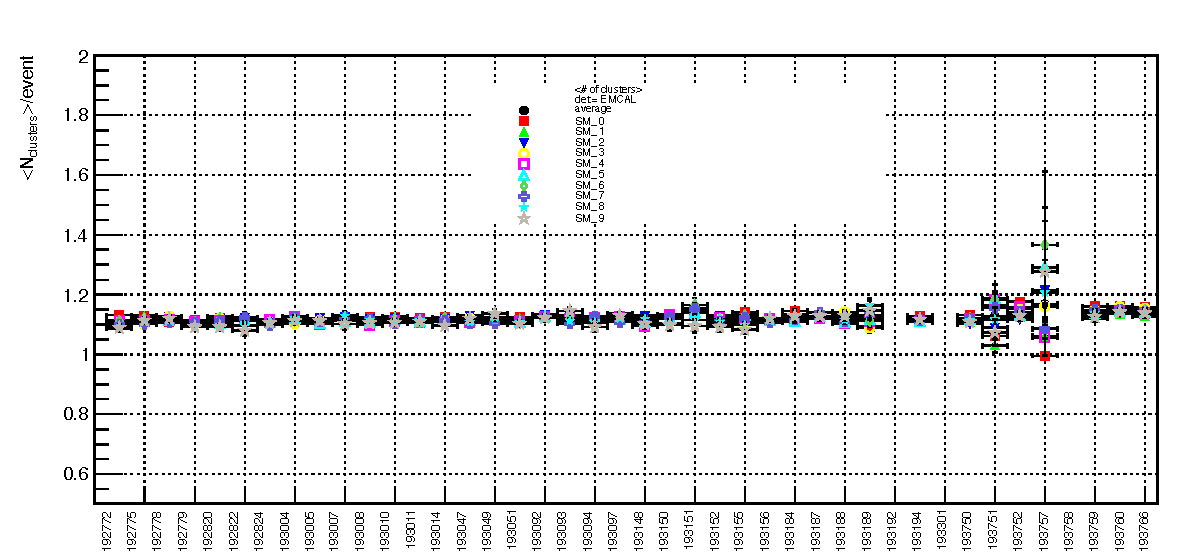
\includegraphics[width=0.9\textwidth]{figures/trendingClusterLHC12iMB.pdf}
\end{center}
\caption{\label{fig:trendingCluster}
Example of trending plot for period LHC12i: mean number of cluster per event as a function of runnumber for MinBias events.}
\end{figure}



{\bf $\pi^0$ Averages: (trendingPi0.C):}

This macro computes some fits over invariant mass histograms and store the fit parameters and $\pi^0$ computed values in a TGraph as a funcion of runnumber. The following histograms are used:
\begin{itemize}
\item EMCAL\_hIM: Invariant mass histogram filled over the whole cluster pairs.
\item EMCAL$\_$hIM$\_$Mod$\_$xx: Invariant mass histogram filled over the cluster pairs in the same supermodule.
\end{itemize}

The fit is  done by a gaussian plus  a 2$^{nd}$ order polinom for background. This is a very ``raw'' fitting wich may not be appropriate especially for the PbPb cases but allows to check the stabilities of averages (mass, width, number of $\pi^O$).



\begin{itemize}
\item Mean number of  $\pi^0$ per event is computed over EMCAL and also per supermodule.
\item Mass of the $\pi^0$ per event is computed over EMCAL and also per supermodule.
\item Witdh of the $\pi^0$ per event is computed over EMCAL and also per supermodule.
\end{itemize}



The use of these set of QA macros allows to identify problematic runs (subperiod with missing part of detectors) or more general features. Also it can be used to check global observables for different dataset used for analysis purpose. 



\subsection{Event display}

\subsection{Logbook tips}